\documentclass[10pt,a4paper,german]{book}
\usepackage[utf8]{inputenc}
\usepackage[german]{babel}
\usepackage{graphicx}
%\usepackage{enumitem}
\author{Peter Silie}
\title{	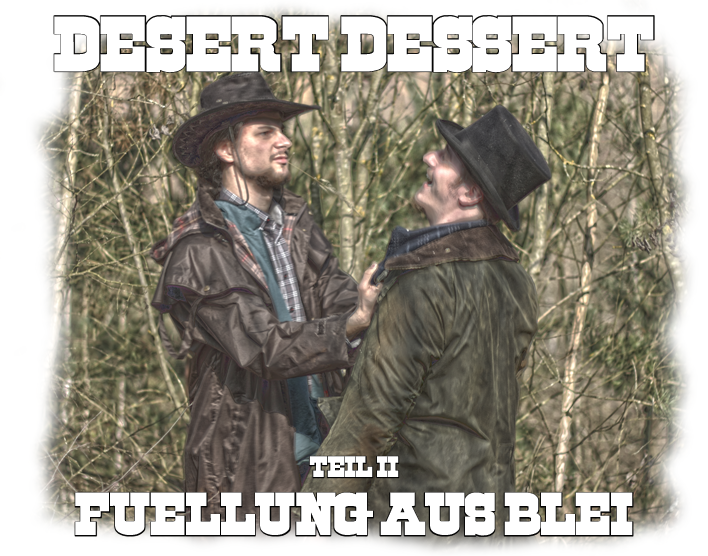
\includegraphics[scale=0.5]{titelbild.png}\\
		\vspace{1cm}
		Desert Dessert\\
		Teil 2\\
		Füllung aus Blei
		}
\date{16.04.2014}

%\setitemize{
%  fullwidth,
%  label=,
%  leftmargin=*,
%  nolistsep
%}

\begin{document}
\maketitle
\tableofcontents
\newpage
\paragraph{Vorwort}
In der Film- und Fernsehwelt erleben wir es wieder und wieder. Teil 2 einer jeden Trilogie dient oft nur als Lückenfüller und um die Leute auf die weiterführende Geschichte in Teil 3 vorzubereiten, obwohl die Geschichte in Teil 1 schon einen guten Abschluss fand.

Dies gilt es hier unter allen Umständen zu vermeiden. Gute Vorarbeit leistete dabei Teil 1, der viele Fragen offen lässt und nur einen kleinen Teil der Krapfenwestern-Welt aufgezeigt hat.
\chapter{Prolog}
\section{Ende Teil 1 - Rache ist süß}
Lückenzahn Bill denkt sich in Sicherheit an einem abgelegenen Ort. Er sitzt auf einem rostigen, alten Rohr und will gerade in den erbeuteten Krapfen beissen, da wird er ihm aus der Hand geschossen. Erschrocken springt er hinter das Rohr und blickt sich langsam in der Richtung um, aus der seiner Meinung nach der Schuss gekommen ist. In der Ferne sieht man Sack'l Mac Joe auf ihn zugehen. Lückenzahn Bill springt auf das Rohr.

\begin{verse}
\textit{\glqq He! Mein Krapfen!\grqq}

Schneller Schwenk auf das Gesicht von Sack'l Mac Joe.

\textit{\glqq Und jetzt werd ich dir eine Füllung verpassen!\grqq}\\
\end{verse}

Er schießt und trifft Lückenzahn Bill, welcher daraufhin zu Boden stürzt. Fade out...
Sack'l Mac Joe nimmt sich den Krapfen aus Lückenzahns kalten, toten Händen, beisst provokativ hinein und geht dem Horizont entgegen.
Der Abspann fliegt durch das Bild.
Am Ende sieht man, dass Lückenzahn Bill nochmals in die Kamera blickt. Es bleibt offen, ob das nun ein Outtake war, ein Lustiges Ende oder ob er noch lebt.

\section{Übersicht Handlung Teil 2 - Füllung aus Blei}

\paragraph{Ausgangssituation.}
    \subparagraph{Sack'l Mac Joe} hat nun 2 Probleme.
    Er kann nicht beweien, dass er Lückenzahn Bill zur Strecke gebracht hat, was nochdazu sehr unklat ist UND er hat Tonys Krapfen gegessen und sich diesen somit zum Feind gemacht.
    \subparagraph{Lückenzahn Bill} ist bei den Indianern untergekommen.
    Er versteckt sich und wartet, bis Gras über die Sache gewachsen ist. Ausserdem tüftelt er an einem Plan, wie er an mehr Krapfen kommen kann.
    \subparagraph{Tony ohne Hut} fährt in die Stadt um sich einen neuen Hut zu besorgen.
    Dabei kommt ihm eine Idee, wie er das Geld seiner Schuldner eintreiben kann.

\paragraph{Anfang.}
    \subparagraph{In die Stadt.}
    \textbf{Tony} fährt in die Stadt um sich einen neuen Hut zu besorgen. Dort angekommen sieht er einen Stecklbrief von Lückenzahn Bill und beschließt ebenfalls ein Kopfgeld auszusetzen, auf \textbf{Sack'l Mac Joe}. Knausrig wie er ist, fällt das Kopfgeld sehr klein aus, weshalb nur ein armer, verrückter Mexikaner namens \textbf{Mexican Kid} darauf anspringt.

\paragraph{Hauptteil.}
    
\subparagraph{Haupthandlung}
    \textbf{Sack'l Mac Joe} stellt fest dass er einen Fehler begangen hat, er hat sich einen reichen Gegner geschaffen und keinen Beweis, dass \textbf{Lückenzahn Bill} tot ist. Er kehrt zum Ort des Geschehens zurück, findet aber keine Leiche. So macht er sich erneut auf die Suche nach seinem ersten Kopfgeldauftrag.
\subparagraph{Nebenhandlung}
    \textbf{Tony} will keine Rache, er will nur sein Geld wieder. So jagt er \textbf{Lückenzahn Bill} und \textbf{Sack'l Mac Joe}. Das größte Hindernis auf seiner Jagt ist sein Geldbeutel. Er will kein Geld ausgeben, schafft sich aber immer mehr und mehr Schuldner.

\paragraph{Schluss.}
    \subparagraph{Dramatische Wendung.}
    \textbf{Lückenzahn Bill} schafft es \textbf{Sack'l Mac Joe} zu überlisten und jagt ihn in eine todsichere Falle.
    \subparagraph{Wer hätte das gedacht.}
    \textbf{Tony} stellt fest, dass man es auch auf ihn abgesehen hat.

\chapter{Drehbuch: Teil 2 - Füllung aus Blei}
\section{Tony fährt in die Stadt}
\end{document}
